\section{Proposed System} \label{section:proposed_system}

In this section, we present how our system can learn to annotate different photos and briefly describe main steps in our BoW model.

\subsection {Learn from manual annotations and automatic annotation for new photos} \label{section:main_flow}

Figure \ref{fig:flow_1} illustrates the overview of our proposed system to automatically recommend personalized annotations for newly uploaded photos. First, a user simply uses his or her smartphone’s camera to capture scenes or objects in real life such as books, dogs, or buildings. A photo is then sent to the annotation server for processing and the server returns the list of visual similar photos. Additionally, each photo attaches a list of annotations and these possible personalized annotations are re-ranked and sent to the user. The user can review and approve these personalized annotations before sharing the photo to social networks such as Facebook, Flickr, or Google Plus along with the approved personalized tags.

Figure \ref{fig:flow_2} shows how our system learns to annotate a photo from samples provided by a user in the past. First, a user manually chooses suitable tags for some photos and these photos along with the tags are then sent to the server. Subsequently, our server process identifies and recommends the user to also apply these changes to visually similar photos in his or her albums. The user can approve before these changes take effect in the database. From this point of time, our system automatically annotates new photos for that user based on these new configurations.

\begin{figure}
    \centering
    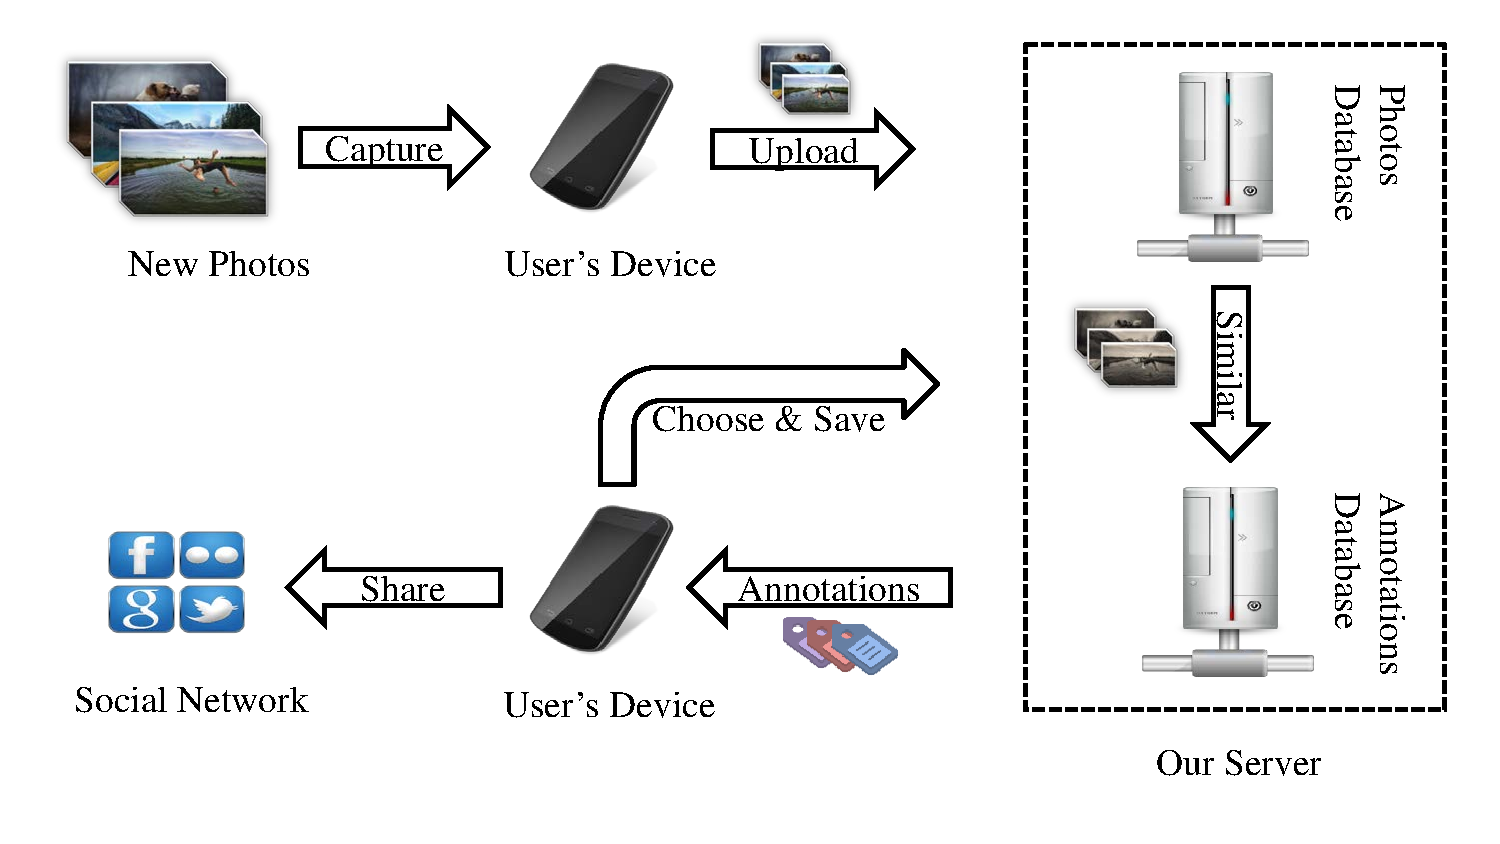
\includegraphics[width=5.0in]{flow1.pdf}
    \caption{Overview of our proposed system to automatically recommend personalized tags.}
    \label{fig:flow_1}
\end{figure}

\begin{figure}
    \centering
    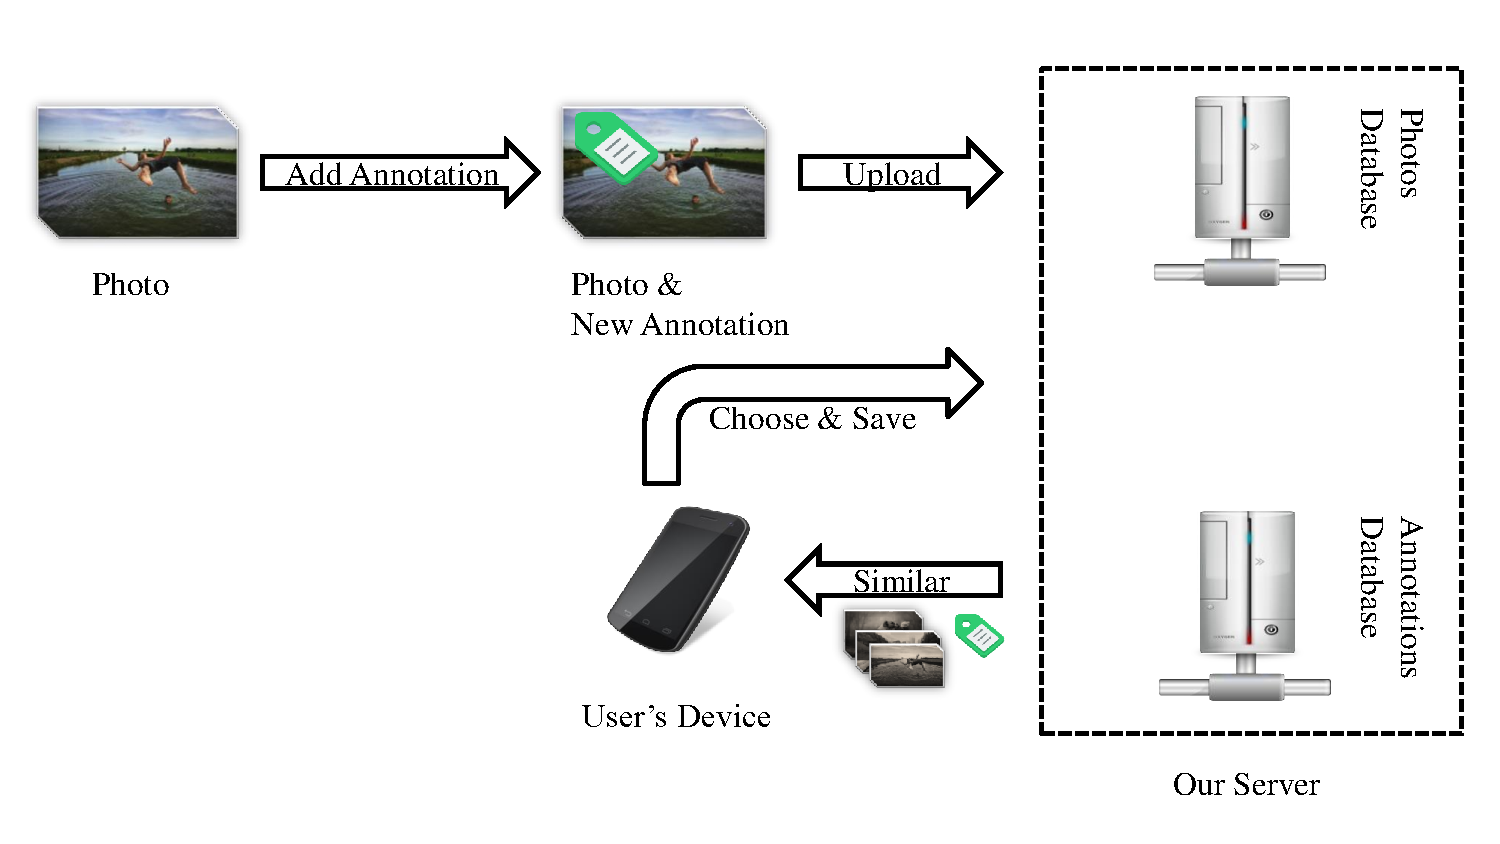
\includegraphics[width=5.0in]{flow2.pdf}
    \caption{Overview on how our system learn to annotate photo from samples provided by users.}
    \label{fig:flow_2}
\end{figure}

\subsection{Visual Instance Search Method} \label{section:visual_search}
\subsubsection{Feature Extraction} \label{section:feature_extraction}

To detect and extract features from images, there are many methods that have been proposed (Harris-Affine, Hessian-Affine detectors \cite{Mikolajczyk2004}, Maximally stable extremal region (MSER) detector \cite{conf/bmvc/MatasCUP02}, Edge-based region detector \cite{Tuytelaars99content-basedimage}, Intensity extrema-based region detector \cite{Tuytelaars00widebaseline} ...). The authors choose to use Hessian-Affine detector, for detecting and extracting features from images. In our version of BoW model, we use Perd'och's implementation of SIFT detector, which is shown to perform best on Oxford Building Dataset \cite{perdoch}.

\begin{figure}
    \centering
    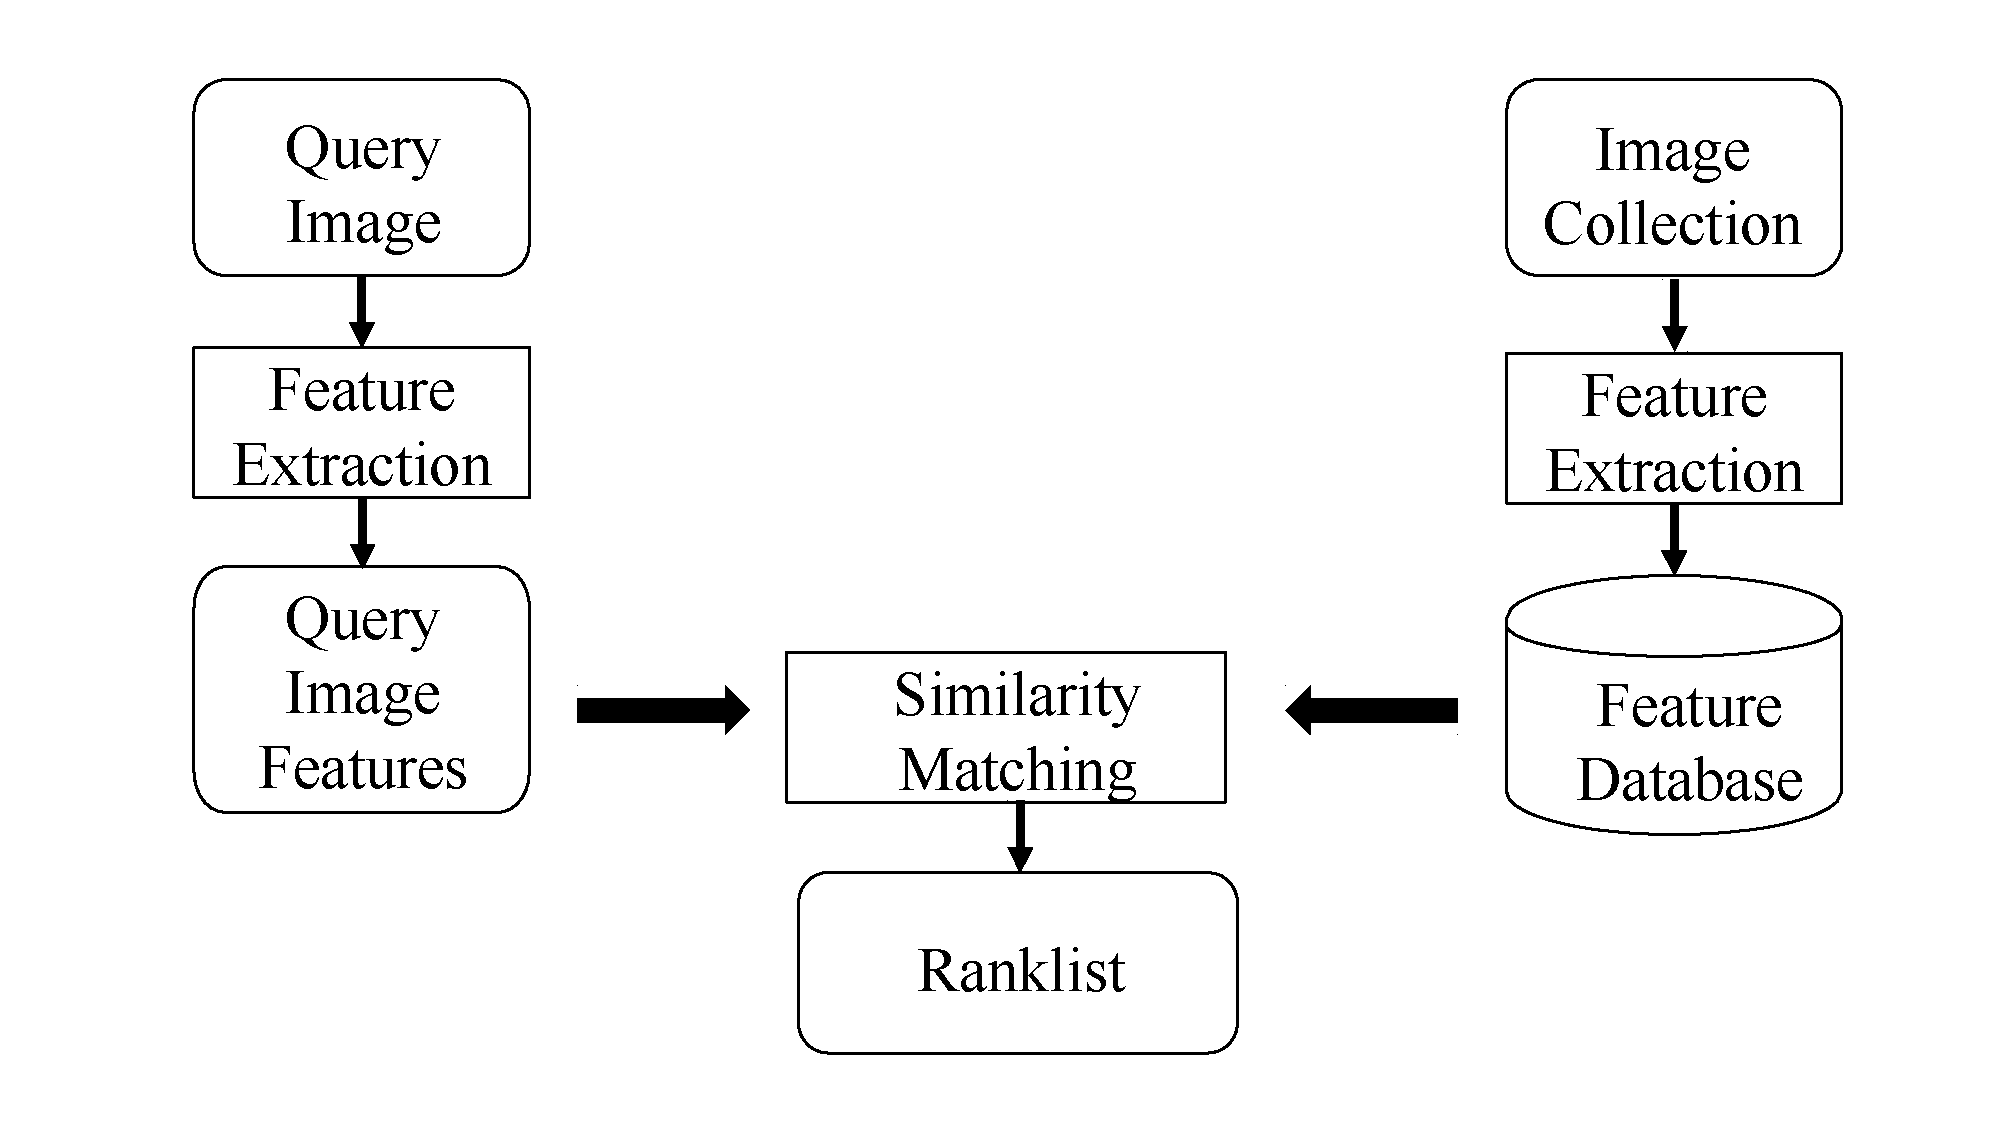
\includegraphics[width=4.0in]{ImageRetrievalSystem_fixed.pdf}
    \caption{How an Image Retrieval System works}
    \label{fig:image_retrieval_system}
\end{figure}

\begin{figure}
    \centering
    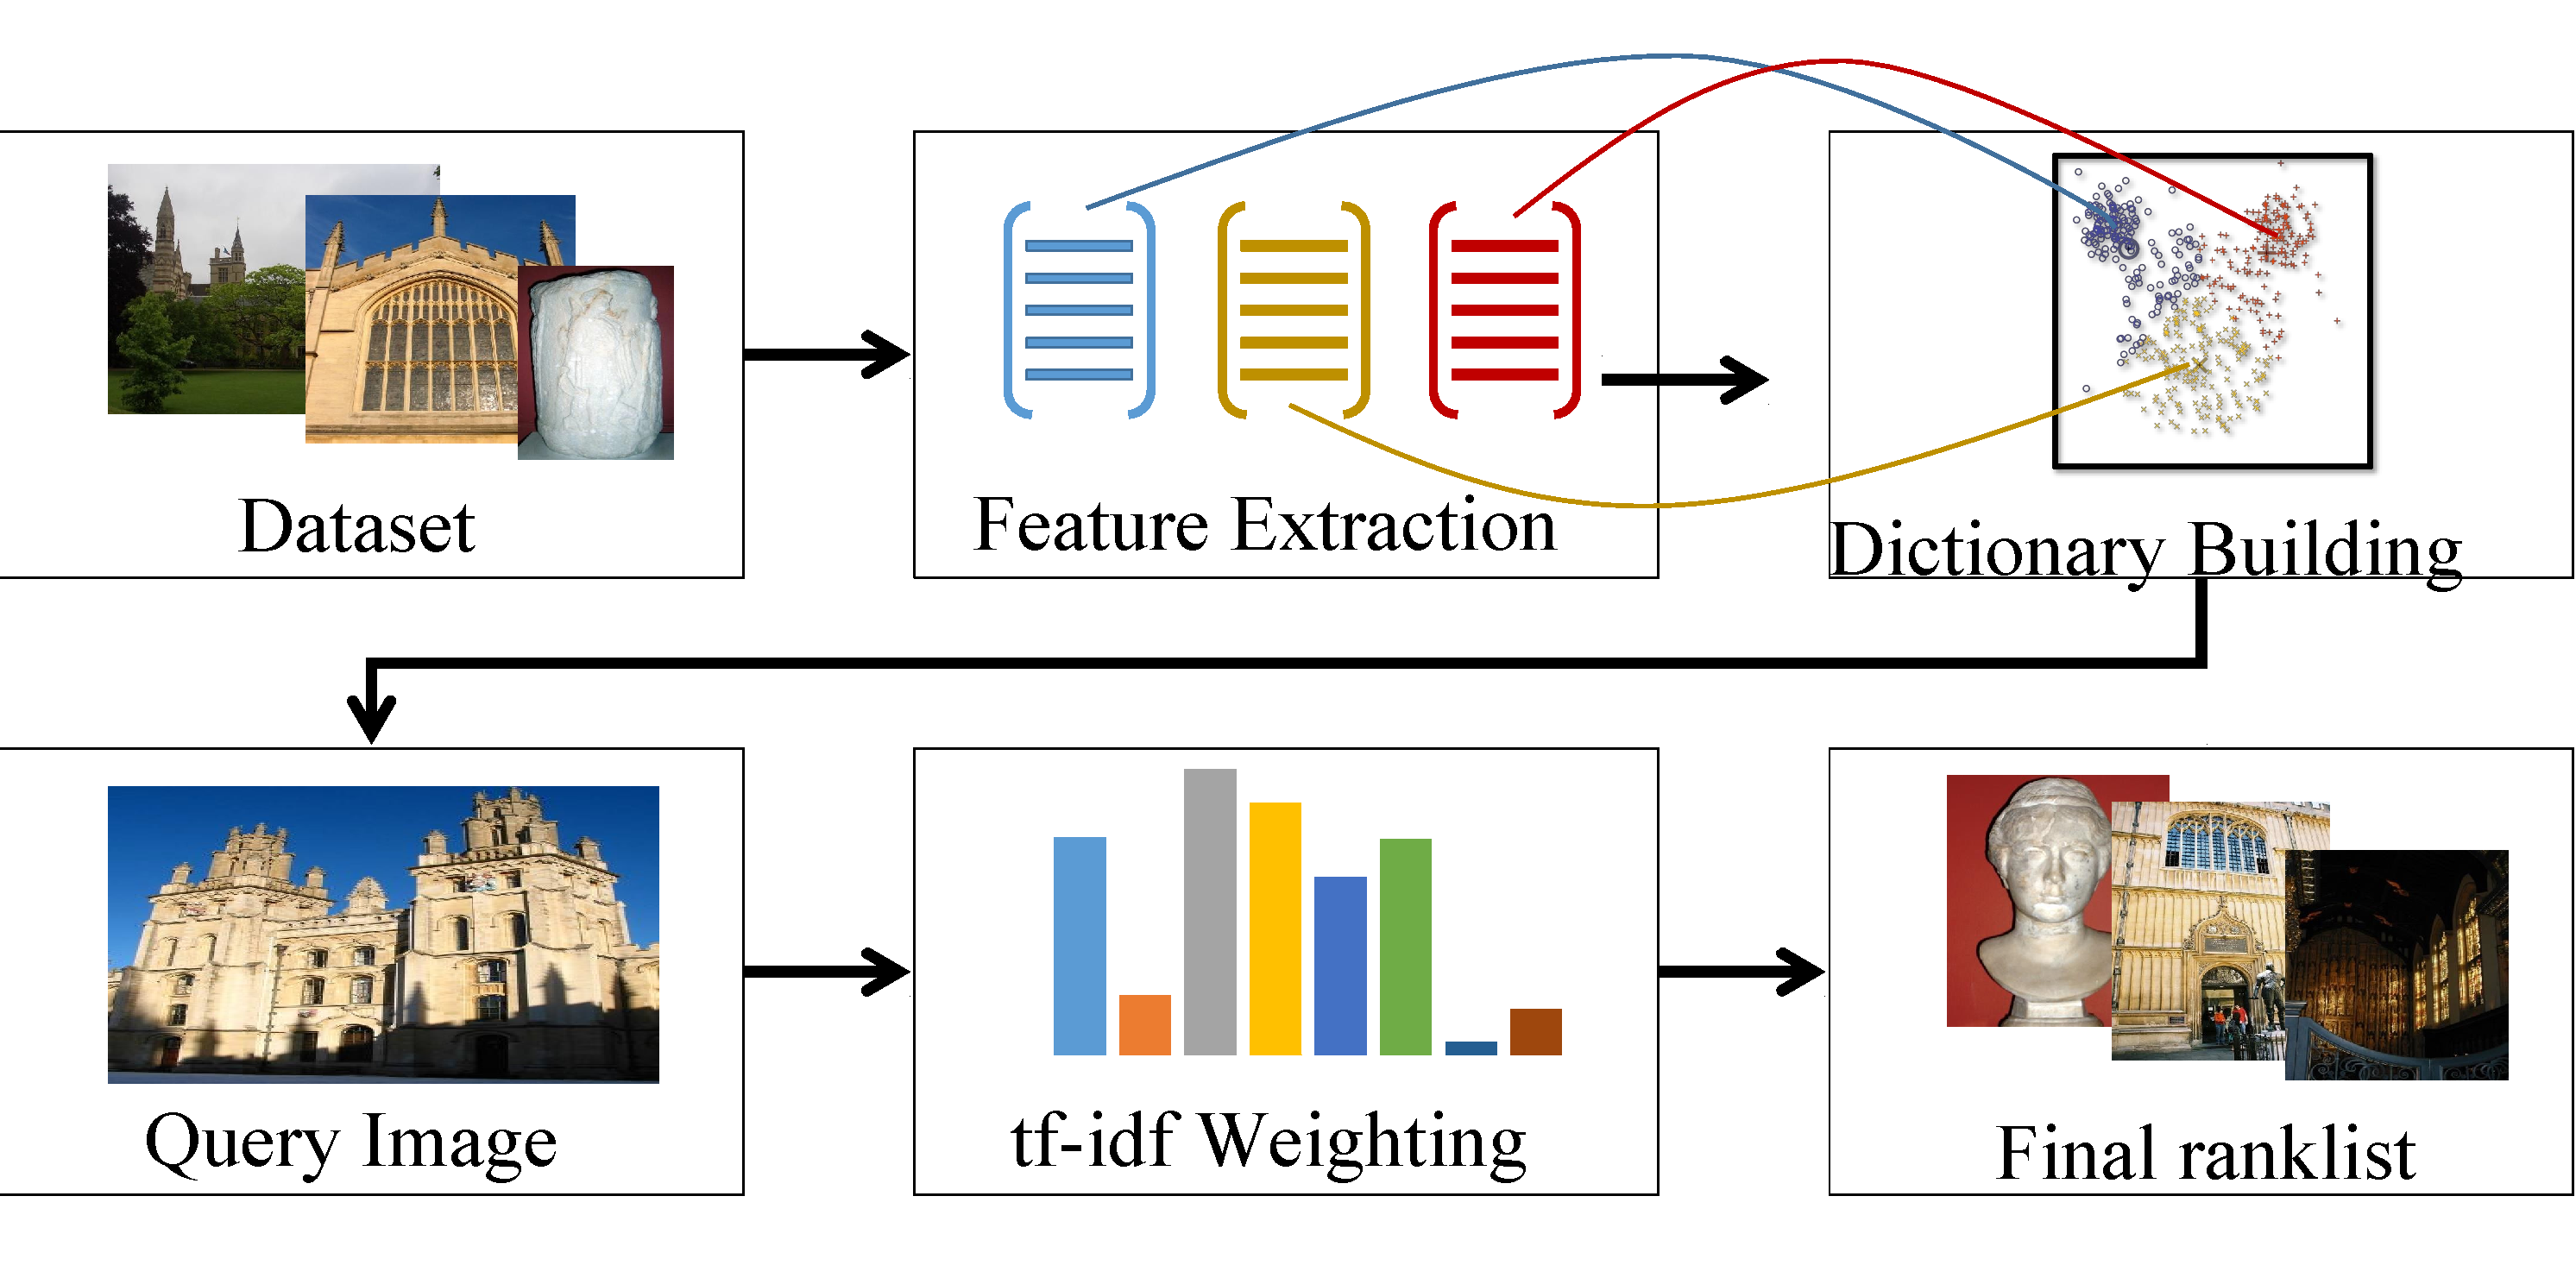
\includegraphics[width=4.0in]{process_fixed.pdf}
    \caption{Proposed framework}
    \label{fig:proposed_framework}
\end{figure}

\subsubsection{Dictionary Building} \label{section:dictionary_building}
Treating each descriptor as an individual visual words in the dictionary results in a worthless waste of resources and time. In order to overcome this obstacle, the authors therefore build the dictionary by considering some similar descriptors as one. In other words, all descriptor vectors are divided into $k$ clusters, each representing a visual word. There are many algorithms that are proposed to solve this kind of problem. However, the authors use the approximate k-means (AKM). AKM is proposed by Philbin et al. \cite{2}. Comparing to the original k-means, AKM can reduce the majority amount of time taken by exact nearest neighbors computation but only gives slightly different result. Also, in \cite{2}, Philbin et al. shows that using 1M dictionary size would have the best performance on the Oxford Building 5K Dataset \cite{oxbuilding}.

\subsubsection{Quantization} \label{section:quantization}

Subsequently, each 128-dimension SIFT descriptor needs to be mapped into the dictionary. Commonly, each descriptor is assigned into the nearest word in the dictionary. Thus, when two descriptors are assigned to different words, they are considered as totally different. In practice, this hard assignment leads to errors due to variability in descriptor (e.g. image noise, varying scene illumination, instability in the feature detection process ...) \cite{7}. In order to handling this problem, the authors use soft assignment instead of hard assignment. In particular, each 128-dimension SIFT descriptor is reduced to a k-dimension vector of their $k$ nearest visual words in the dictionary. Each of these $k$ nearest cluster is assigned with weights calculated from the formula proposed by Sivic et al. \cite{7}, $weight = \exp(-\frac{d^2}{2\delta^2})$, where $d$ is the distance from the cluster center to descriptor point. Then, by adding all these weights to their corresponding bins, we have the BoW representation of an image.

In this work, $k$ and $\delta^2$ are chosen to be 3 and 6250, respectively.

\subsubsection{tf-idf Weighting Scheme} \label{section:tfidf_weighting}

As mentioned in section \ref{section:background_relatedworks}, tf-idf is a popular weighting scheme that is used by almost any BoW model. In this section, the authors show how this scheme is applied to our system.

For a term $t_{i}$ in a particular document $d_{j}$, its term frequency $tf_{i, j}$ is defined as follow:

\begin{equation} 
        tf_{i, j} = \frac{n_{i, j}}{\sum\limits_{k} n_{k, j}}
\end{equation}
Where $n_{i, j}$ is the number of occurrences of the considered term $t_{i}$ in the document $d_{j}$. The denominator is the sum of the number of occurrences of all the terms in document $d_{j}$.

The inverse document frequency $idf_{i}$ of a term $t_{i}$ is computed by the following formula:

\begin{equation}
        idf_{i} = \log{\frac{\left|D\right|}{\left|\{j: t_{i} \in d_{j}\}\right|}}
\end{equation}
Where, $\left|D\right|$ is the total number of documents in the corpus, $\left|\{j: t_{i} \in d_{j}\}\right|$ is the number of documents where the term $t_{i}$ appears, i.e. $n_{i, j} \ne 0$

The tf-idf weight of a term $t_{i}$ in a document $d_{j}$ is then calculated as the product of tf and idf:

\begin{equation}
{tfidf}_{i, j} = tf{i, j} \times idf_{i}
\end{equation}

The tf-idf weight is then used to compute the similarity score between an image $d_{i}$ and a query $q$:

\begin{equation}
s_{d_{i}, q} = \vec{{tfidf}_{i}} \cdot \vec{{tfidf}_{q}} = \sum\limits_{j = 1}^{\left|T\right|} {tfidf}_{i, j} \times {tfidf}_{q, j}
\end{equation} 

Finally, by sorting the list of images corresponding to their similarity score with a query, we achieve the raw ranked list of this query which is then used for the Spatial Rerank step.
